\documentclass[10pt]{article}


\usepackage[a4paper , left=31.7mm, top=25.4mm]{geometry}
\usepackage{hyperref}
\hypersetup{
	colorlinks=true,
    linkcolor=blue,
    filecolor=magenta,      
    urlcolor=cyan,
    pdftitle={Overleaf Example},
    pdfpagemode=FullScreen,
}
\setlength\parindent{0pt}
\usepackage{listings}
% Copyright 2017 Sergei Tikhomirov, MIT License
% https://github.com/s-tikhomirov/solidity-latex-highlighting/

\usepackage{listings, xcolor}

\definecolor{verylightgray}{rgb}{.97,.97,.97}

\lstdefinelanguage{Solidity}{
	keywords=[1]{anonymous, assembly, assert, balance, break, call, callcode, case, catch, class, constant, continue, constructor, contract, debugger, default, delegatecall, delete, do, else, emit, event, experimental, export, external, false, finally, for, function, gas, if, implements, import, in, indexed, instanceof, interface, internal, is, length, library, log0, log1, log2, log3, log4, memory, modifier, new, payable, pragma, private, protected, public, pure, push, require, return, returns, revert, selfdestruct, send, solidity, storage, struct, suicide, super, switch, then, this, throw, transfer, true, try, typeof, using, value, view, while, with, addmod, ecrecover, keccak256, mulmod, ripemd160, sha256, sha3}, % generic keywords including crypto operations
	keywordstyle=[1]\color{blue}\bfseries,
	keywords=[2]{address, bool, byte, bytes, bytes1, bytes2, bytes3, bytes4, bytes5, bytes6, bytes7, bytes8, bytes9, bytes10, bytes11, bytes12, bytes13, bytes14, bytes15, bytes16, bytes17, bytes18, bytes19, bytes20, bytes21, bytes22, bytes23, bytes24, bytes25, bytes26, bytes27, bytes28, bytes29, bytes30, bytes31, bytes32, enum, int, int8, int16, int24, int32, int40, int48, int56, int64, int72, int80, int88, int96, int104, int112, int120, int128, int136, int144, int152, int160, int168, int176, int184, int192, int200, int208, int216, int224, int232, int240, int248, int256, mapping, string, uint, uint8, uint16, uint24, uint32, uint40, uint48, uint56, uint64, uint72, uint80, uint88, uint96, uint104, uint112, uint120, uint128, uint136, uint144, uint152, uint160, uint168, uint176, uint184, uint192, uint200, uint208, uint216, uint224, uint232, uint240, uint248, uint256, var, void, ether, finney, szabo, wei, days, hours, minutes, seconds, weeks, years},	% types; money and time units
	keywordstyle=[2]\color{teal}\bfseries,
	keywords=[3]{block, blockhash, coinbase, difficulty, gaslimit, number, timestamp, msg, data, gas, sender, sig, value, now, tx, gasprice, origin},	% environment variables
	keywordstyle=[3]\color{violet}\bfseries,
	identifierstyle=\color{black},
	sensitive=false,
	comment=[l]{//},
	morecomment=[s]{/*}{*/},
	commentstyle=\color{gray}\ttfamily,
	stringstyle=\color{red}\ttfamily,
	morestring=[b]',
	morestring=[b]"
}

\lstset{
	language=Solidity,
	backgroundcolor=\color{verylightgray},
	extendedchars=true,
	basicstyle=\footnotesize\ttfamily,
	showstringspaces=false,
	showspaces=false,
	numbers=left,
	numberstyle=\footnotesize,
	numbersep=9pt,
	tabsize=2,
	breaklines=true,
	showtabs=false,
	captionpos=b
}

\usepackage{tikz}







\title{Viral-Next Gen Social Communication Tool}
\date{15 January 2022}
\author{Joby Reuben\\jobyreuben@gmail.com}


\begin{document}




\maketitle

\section{Abstract}
This is a Sample Abstract of the Viral Project.

\section{User Problems \& Basic Solutions}
This is a Sample Problems of the Viral Project.

\section{Vision Statement}
To bring blockchain \& crypto adoption to the masses we would got to bridge social communication with defi and tokenised economy. The Viral Network of Applications standards are designed in such a way that our vision to bring an proficient, user-friendly mobile application will combine several divisions of decentralized protocols that can lead to an ultimate tool for crypto acknowledgement. The divisions which we are focussing to rebuild is listed\\
\\
\textbf{\large Social Media}
\begin{enumerate}
\item To create a Real-world Decentralised Social Media
\item To construct an Autonomous self-evolving platform
\item To construct an Interactive Next-Gen Social Media
To form a clean people-owned platform appropriate for all age groups
\end{enumerate}
\textbf{\large Crypto Adoption}
\begin{enumerate}
\item To provide people to hop into crypto from fiat effortlessly \& securely
\item To give access to use cryptocurrencies to internet people without investing
\item To bring all major crypto for individuals to adapt rapidly using a single wallet
\end{enumerate}
\textbf{\large NFT \& Metaverse}
\begin{enumerate}
\item To democratize NFTs to Masses
\item To kickstart Metaverse adoption
\end{enumerate}
\textbf{\large Blockchain}
\begin{enumerate}
\item To supply the utmost speed of transactions through On-Chain \& Off-Chain solutions
\item To Develop a feeless, fast, Zero Inflation, Deflationary, smart contract chain
\end{enumerate}

\section{Unified Mobile Application - An Intro to Viral}

\hyperlink{https://sample.com}{App Brouchure}\\

\textit{Images}\\

A Next-Gen Social Media platform bridging interactive media, NFTs, and blockchain technologies' underlying applications into an every-day user-based mobile app. Viral bridges Social Media with Blockchain, Wallets, Exchanges and NFT Markeplaces to bring the ultimate one-app for the common masses to adopt into the tokenised economy.\\

Every media shared on viral is an unique NFT where it can be utilized to create limitless achievable outcomes across the platform. Users can share ultra-short to short videos, thoughts through text, sell NFTs and additionally make communication between one-on-one, private groups and, open channels with total genuine privacy. App users will be benefitted from zero ads, cryptographic encryption, censorship-resistant and, also get to use various cryptocurrencies throughout the platform. Every user is an active contributor to the platform by which they receive rewards (payment) in Viral Coin for effectively utilizing the Viral Application and it's child platforms.\\

\section{Viral Platform Architecture}

\begin{enumerate}

\item \textbf{Viral App}: Decentralized Social Media Platform bridging Blockchain applications for limitless possibilities.

\item \textbf{Viral Smart Chains}: Horizontally Scalable EVM Smart Chain on Top of IOTA's Tangle.

\begin{enumerate}

	\item \textbf{Payment Channels (L2)}: State Channels to move value off-chain for lightning fast micro-transactions.

	\item \textbf{Zk-Rollups (L2)}: Batching Multiple Off-chain NFT Standard Tokens (ERC721) to On-Chain,
	\item \textbf{Viral Bridge}: Interopability of various major cryotocurrencies by wrapping tokens decentralized such as Bitcoin, Ethereum,etc into Viral Smart Chains.
	\item \textbf{Horizontal Chains}: Additional of New Chains anchored to IOTA Tangle that communicates between multiple Viral Smart Chains for unlimited scaling

\end{enumerate}
	
Viral Bridge: Interopability of various major cryotocurrencies by wrapping tokens decentralized such as Bitcoin, Ethereum,etc into Viral Smart Chains.
Horizontal Chains: Additional of New Chains anchored to IOTA Tangle that communicates between multiple Viral Smart Chains for unlimited scaling

\end{enumerate}


Smart Wallet : Viral's App's built in Non-Custodial Viral Smart Chain compatible hot wallet that allows user to send \& hold tokens, mint NFTs and receive rewards.

Viral CEX-Centralized Exchange: Trustless Non-Custodial Exchange for Fiat-Crypto trading
Viral DEX-Decentralized Exchange: Automated Market Making Protocol for exchanging Viral tokens
P2P Exchange: Trustsless anonymous exchange leveraging Peer-to-Peer protocol
Viral Name System: Decentralized blockchain based username protocol for transfers instead of cryptographic public address.
Child Platforms: Independant platforms anchored to the viral network for effective improvement of protocols

Dev-Space: Application for Developers to decide on reward allocation for improving Viral-Beta
ROV App: Curator Platform to vote and remove reported content on Viral-Alpha
Ad Platform: Decentralized Ad platform connecting Influencers,businesses and users for trustless engagement-proof ads.
Reward Pool: To incentivize all users, miners, developers using smart contracts for their content, validation of transactions, and continuous development through unbiased pointing strategy that offers more rewards to bigger contributors.

Other Backend: For contingencies which will be later decentralized in the further phases of the development roadmap



%Test Javascript Program



%Test Solidity Program

\begin{lstlisting}[language=Solidity, caption={Sample}]

// SPDX-License-Identifier: MIT
// compiler version must be greater than or equal to 0.8.10 and less than 0.9.0

pragma solidity ^0.8.10;

contract HelloWorld {

    string public greet = "Hello World!";
    
}

\end{lstlisting}

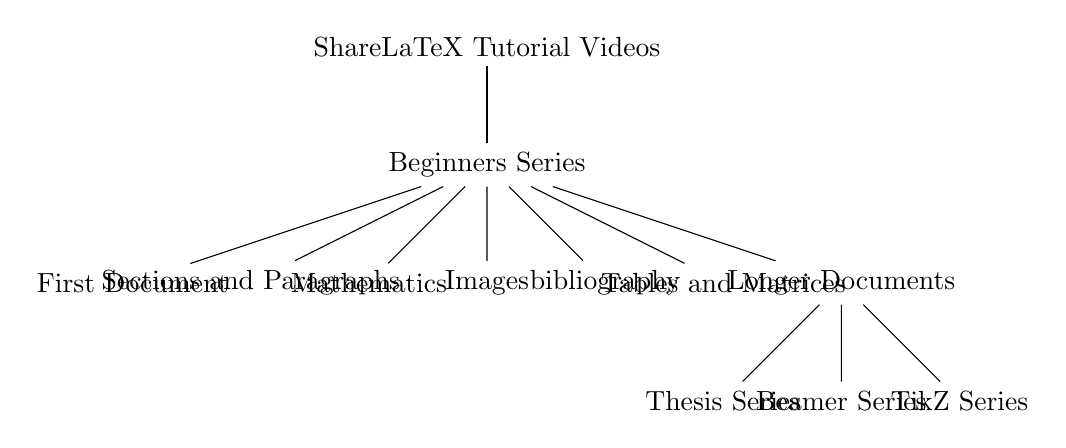
\begin{tikzpicture}

\node{ShareLaTeX Tutorial Videos}
	child { node {Beginners Series}
		child { node {First Document}}
		child { node {Sections and Paragraphs}}
		child { node {Mathematics}}
		child { node {Images}}
		child { node {bibliography}}
		child { node {Tables and Matrices}}
		child { node {Longer Documents}}		
	}
	
	child { node {Thesis Series}}
	child { node {Beamer Series}}
	child { node {TikZ Series}}
;
\end{tikzpicture}























\end{document}



